\documentclass[12pt,english]{article}

\usepackage{natbib}

\usepackage{graphics,graphicx,dcolumn,bm,fleqn,epic,eepic,float}
\usepackage{amssymb,amsmath,multirow,rotate,rotating,color}
\usepackage[utf8]{inputenc}

\usepackage[english]{babel}
\usepackage{caption}
\usepackage{subcaption}
\usepackage{tikz}
\usepackage{hyperref}
\hypersetup{
    colorlinks=true,
    linkcolor=blue,
    filecolor=magenta,      
    urlcolor=cyan,
}
%\usepackage[usenames,dvipsnames,svgnames,table]{xcolor}
\tikzset{fontscale/.style = {font=\relsize{#1}}}
\usetikzlibrary{calc}
\makeatother

\newcommand{\figref}[1]{Fig.~\ref{fig:#1}}
\newcommand{\eqnref}[1]{Eq.~(\ref{eq:#1})}
\newcommand{\ts}{\textsuperscript}

\definecolor{tuered}{RGB}{214,0,74}

\newcommand{\todo}[1]{\textbf{\textcolor{tuered}{ TODO: #1}}}

\newcommand{\vectornorm}[1]{\left|\left|#1\right|\right|}

\renewcommand{\vec}[1]{\mathbf{#1}}
\newcommand{\uvec}[1]{\hat{\vec{#1}}}
\newcommand{\tensor}[1]{\mathbf{#1}}

\definecolor{pyblue}{HTML}{1F77B4}
\definecolor{pyorange}{HTML}{FF7F0C}
\definecolor{pygreen}{HTML}{2CA02C}
\definecolor{pyred}{HTML}{D62728}

\begin{document}

% The referee PDF has been generated from r239 -- 'make referee' command.

\section*{Reply to Referee two}

We thank the Referee for his/her comprehensive feedback on our paper 
and for the time and effort he/she spent for its careful review. 
We are glad to read that he/she finds the paper interesting and the results valuable. We believe that addressing the Referee's remarks
indeed helped us to significantly improve the manuscript quality.
We have prepared a detailed list of answers to all Referee's comments. 
All changes in the paper are edited in red colour, for the sake 
of easier readability. 
 
\begin{itemize}


\item[ \textbf{\underline{Comment 1.}}]
{
With respect to the mobility function, I think the paper requires some references and clarifications. This form is not the usual one. 
The paper of Haley and Miksis~\cite{Haley_Miksis_1991} considers several possibilities for the slip coefficient $\lambda(h)$ for its eq. (2.22). 
The usual one is treating $\lambda$ as a constant~\cite{gonzalezStabilityLiquidRing2013}. 
This case accounts for the second term of the denominator of eq. (2) in this paper. 
Haley and Miksis discuss the differences in the results when selecting other different models for $\lambda(h)$ including one that goes as $\lambda=\lambda_1/h$ that accounts for the third term in the denominator of (2). 
However, we have a mixture of both cases in this paper. 
This means that some further discussion is needed when comparing the results here with those of previous works. 
I wonder why the authors did not consider first the case of constant $\lambda$ since the comparisons are made against an approximate LSA result that uses this assumption. 
The inclusion of the other law will alter some results making more difficult to assess the origin of any discrepancy.


\item[ \textbf{Answer}]
{
We thank the Referee for this useful and interesting remark. We agree, indeed, that our model for the mobility 
function mixes, somehow, a pure Navier's slip condition with that of an effectively $h$-dependent slip length. 
We did not introduce the quadratic term, however, to complicate the theoretical picture, but rather as a further 
regularization of the contact line singularity. Given that the 'slip length' $\delta$ was always kept in the range 
$\delta < h_0$ (the maximum of the height field in the initial condition), we did not expect a major effect, 
at least qualitatively, on the results. Motivated by the Referee's comment, though, we have made a test removing 
the quadratic term from the $\alpha(h)$, i.e. corresponding to the more standard mobility function 
\begin{equation}\label{eq:mob2}
M(h)= \frac{1}{\mu}\left(\frac{h^3}{3} + \delta h^2\right).
\end{equation}
The results concerning the number of droplets vs initial aspect ratio (for a uniform substrate with $\theta_0 = 20^{\circ}$) are reported in figure~\ref{fig:diff_slip_20deg} and 
compared with the data reported in the paper.
\begin{figure}
    \centering
    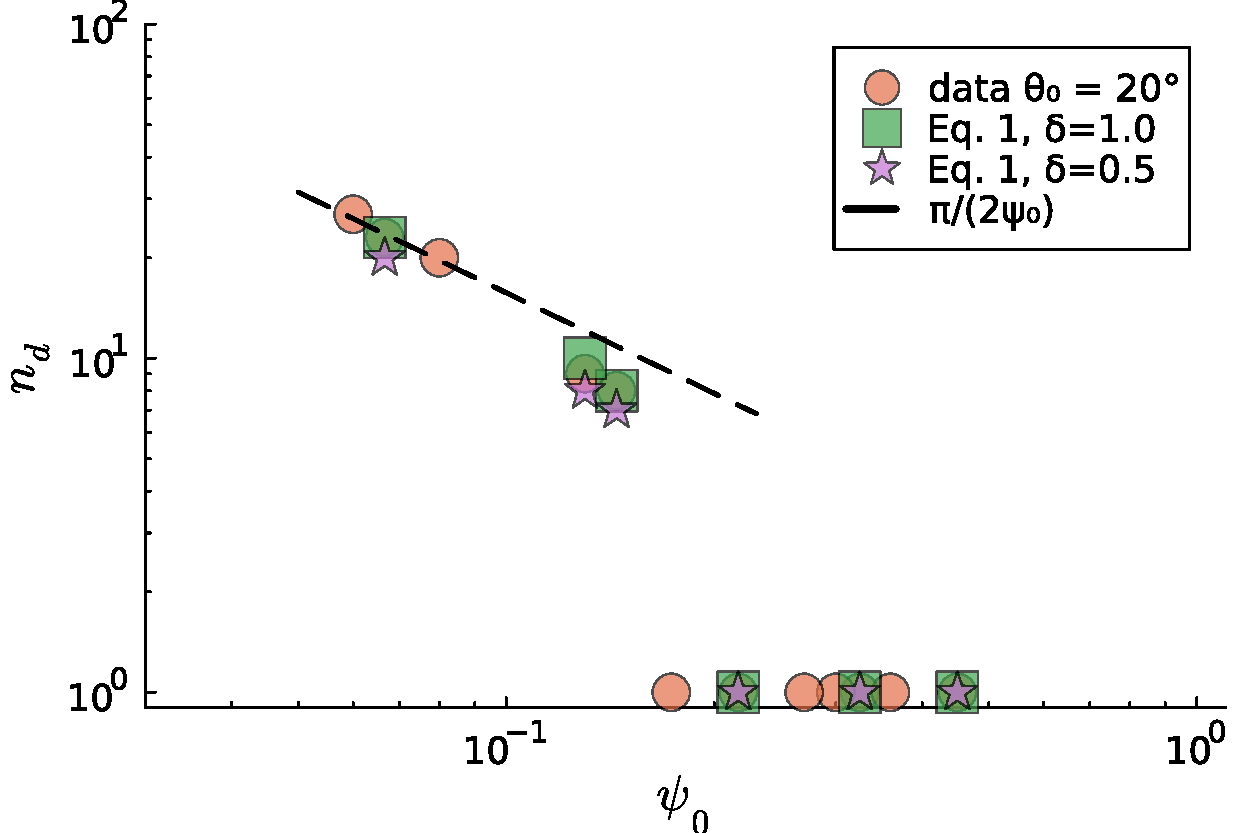
\includegraphics[width=0.85\linewidth]{Ndrops_slip_model.pdf}
    \caption{Figure 2 of the original contribution only plotting the data for $\theta=20^{\circ}$ simulations.
    The green boxes and the purple stars are selected initial conditions with the mobility function given by eq.~\ref{eq:mob2}.
    Both in the collapse and the breakup regime we find reasonable agreement with the original simulations.
    }
    \label{fig:diff_slip_20deg}
\end{figure}
We do not observe indeed a relevant mismatch and we can, therefore, safely assume that possible particular effects 
should not be ascribed to the form of the mobility function.
We have commented on this aspect in Appendix A and we have rephrased the text relative to the mobility in the revised version as follows:\\
\\
\textcolor{red}{The mobility function reads:
\begin{equation}\label{eq:slip}
M_{\delta}(h) = \frac{1}{\mu}\left(\frac{h^3}{3} + \delta h^2 +\frac{\delta^2}{2} h\right),
\end{equation}
where $\delta$ is the slip length. In Equation (\ref{eq:slip}) we have introduced a linear in $h$
(quadratic in $\delta$), in order to strengthen the regularization of the contact line singularity.  
The resulting expression can be recast into the standard form of the mobility
arising from the usual Navier's slip boundary condition at the solid substrate, with an $h$-dependent 
effective slip lengths~\cite{Haley_Miksis_1991,Greenspan1978} (see Appendix A for further details and for numerical values of the parameters).
}
}

\item[ \textbf{\underline{Comment 2.}}]
The other point is the simultaneous inclusion of the disjoining pressure term of eq. (4) with the slipping model. The slipping model allows for an equilibrium while the disjoining term does not, as explained in~\cite{gonzalezStabilityLiquidRing2013}. This leads to the question whether it is possible to reach an equilibrium as stated in section 2.1. If that is the case it should be shown that it is reached before the breakup or collapse dominate the evolution. For example, the authors could show that their simulations reach the analytical equilibrium solution in section 3.1 of~\cite{gonzalezStabilityLiquidRing2013} when disjoining pressure is not considered. This serves as a check that the simulation with their lattice Boltzmann method does not introduce nothing strange to the problem. Moreover, if the full system does not reach any equilibrium soon enough, some of the results may depend strongly on the initial condition. Does a change in the initial form of the profile change the results?
}

\item[ \textbf{Answer}]
{
The Referee is right. We apologize for using the inappropriate term "equilibrium" and
we acknowledge that, indeed, the sentence was confusing and did not clearly explain how we initialize
 the system. 
We have changed the paragraph as follows:\\
\\
\textcolor{red}{A Gaussian noise with zero mean and variance $10^{-4}r_0^2 \sin^2\theta_0$ is also added as an initial perturbation to the interface.}\\
\\
Moreover, as suggested by the Referee, we have checked how the code deals with the actual equilibrium solution 
of~\cite{gonzalezStabilityLiquidRing2013}, upon removal of the disjoining pressure. 
\begin{figure}
    \centering
    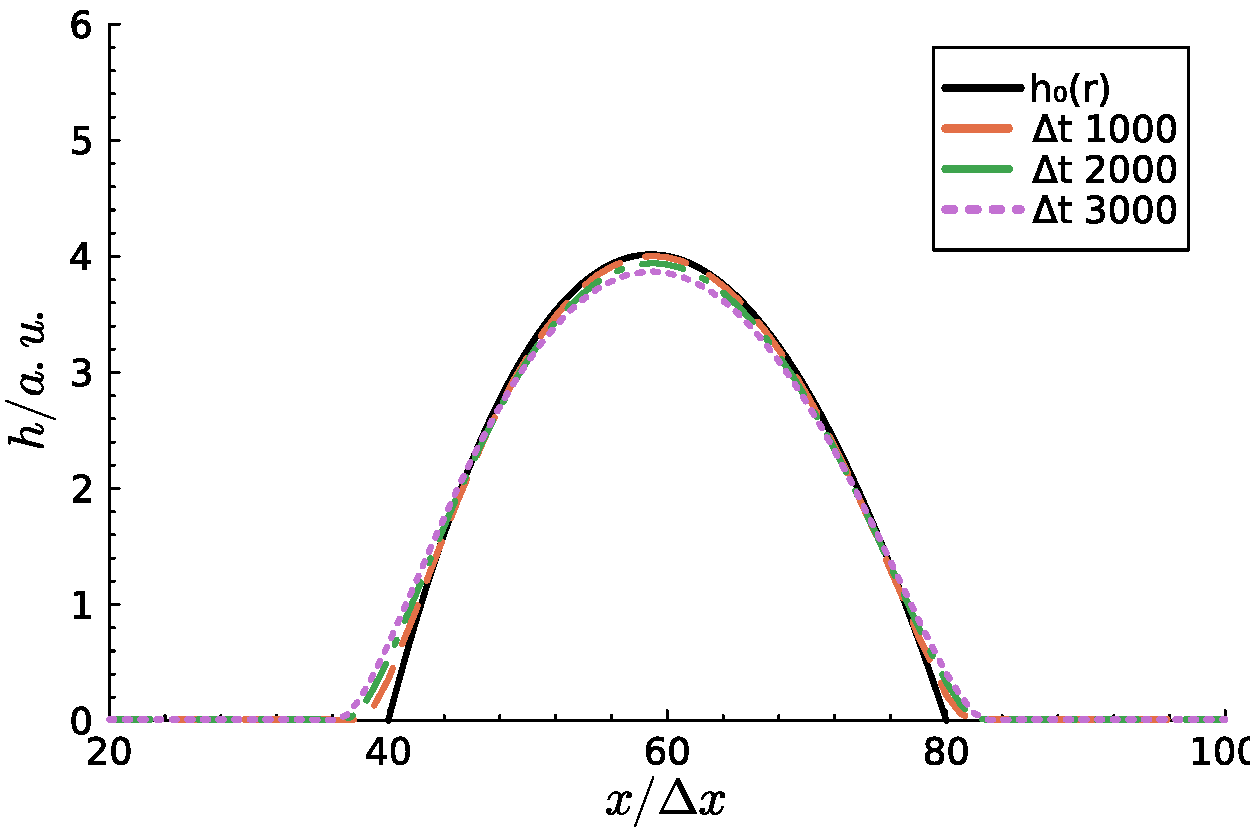
\includegraphics[width=0.85\linewidth]{h0_sim.pdf}
    \caption{The equilibrium solution derived by Gonz\'alez et al. for $R=80$, $r=40$ and $\theta=20$ shown in black.
    The three additional lines depict an evolving thin film without disjoining pressure contribution which has been initialized with the equilibrium solution.}
    \label{fig:h0eq}
\end{figure}
}
The results are reported in figure \ref{fig:h0eq}, where we show the height profile at various instants of time. 
At $t=0$, the initialized profile $h_0(r)$ is Equation (3.5) of~\cite{gonzalezStabilityLiquidRing2013}. The 
profile remains stable, confirming that the numerical method indeed solves the correct equation of motion without 
introducing any artifact. 

\item[ \textbf{\underline{Comment 3.}}]
{
Firstly, they restrict the discussion to an approximate LSA result which is expected to work well for small aspect ratios and large mean radii, but they neglect the more detailed analysis made in~\cite{gonzalezStabilityLiquidRing2013} for higher aspect ratios and different mean radii. 
Note that the stability depends on both parameters, but the authors do not mention the second one. 
In fact, I am not sure which is the value of the mean radius, $r_m$ in the simulations. 
The comparison with an approximate formula for very large $r_m$ is lacking some interesting results in fig. 16 of~\cite{gonzalezStabilityLiquidRing2013} that show an abrupt change in the number of drops for large aspect ratios with respect to the approximate formula. 
This is quite similar to the results shown in fig 2 of this paper. 
Note that the aspect ratio defined in section 3.1 of the submitted paper is a bit different from that used in~\cite{gonzalezStabilityLiquidRing2013}. 
It is related to the initial state in the present paper, while it is the aspect ratio of the equilibrium in Gonz\'alez et al. 
Therefore, the statement made by the authors that "the theory leading to (6) does not account for the disjoinin pressure" (sic, note the typo) is misleading. 
The approximate formula may not account for the results but the underlying LSA theory of the simple slip model could explain the results even if the disjoining pressure term is absent.
Moreover, Gonz\'alez et al. discussed the relation of disjoining pressure and slip models. 
How are the present results related to those for disjoining pressure in~\cite{gonzalezStabilityLiquidRing2013}?
}

\item[ \textbf{{Answer}}]
{
We apologize for not giving explicit values of the mean radius $r_m$ ($R_0$ in our notation). We provide now this information in the Appendix A.
Concerning possible effects due to a potentially "small" $R_0$, this is in principle a good point. 
We remark, however, that the abrupt curve collapse in Fig. 16 of~\cite{gonzalezStabilityLiquidRing2013}
occurs for $\psi_0 > 0.8$, way beyond the value observed in our Fig. 2 ($\psi_0 \approx 0.2$). Moreover, in our case 
all $R_0$ values (in units of $h_0^{(\text{max})}$, i.e. the maximum initial rivulet height) are comparatively large, 
 lying in the range $R_0/h_0^{(\text{max})} \in (10, 600)$; with reference to Fig. 16 of~\cite{gonzalezStabilityLiquidRing2013}, this means that our data are always above the case $r_m =4$ (for which the abrupt 
 change occurs at $\psi_0 \approx 0.92$).
 We believe, then, that we can safely assume to be in the large mean radius limit and that the effect that we observe
 is of different nature. 
 We agree with the Referee that we should discuss our results also under the light of the comparison with the disjoining 
 pressure model done in \cite{gonzalezStabilityLiquidRing2013}. Similar to our findings, they observe that for small 
 $\psi_0$ the agreement with the LSA result is good, whereas, as $\psi_0$ increases, the number of droplets tends to be 
 smaller than the theoretical expectation.
 We have rephrased the discussion around Eq. (6), in order to take into account all these interesting aspects, 
 as follows:\\
\\
\textcolor{red}{For small aspect-ratios, the number of droplets is large ($n_d \gg 1$), 
indicating that the rivulet undergoes a breakup, and decreases with $\psi_0$ following, approximately, the formula 
\begin{equation}\label{eq:maxDrops}
    n_d \approx \frac{\pi}{2\psi_0},
\end{equation}
(dashed line in Fig. 2) derived from linear stability analysis (LSA), assuming that the most unstable mode determines the number of droplets~\cite{gonzalezStabilityLiquidRing2013}.
As $\psi_0$ increases, the agreement tends to deteriorate, with the number of droplets being smaller than the theoretical expectation, in analogy to what reported by Gonz\'alez 
et al~\cite{gonzalezStabilityLiquidRing2013} when comparing numerical results from a disjoining pressure model with the LSA prediction. 
For $\psi_0 \gtrsim 0.2$ we get $n_d=1$, indicating the retractive collapse to a single central droplet; the data 
drop in the number of droplets at $\psi_0 \approx 0.2$, is rather abrupt. From the theoretical analysis of a slip model, a similar behaviour is suggested to be favoured by a small initial main radius $R_0$~\cite{gonzalezStabilityLiquidRing2013}. In that case, however, the curve collapse occurs for much larger values of $\psi_0$ ($\psi_0 >0$). Moreover, our simulations are in the large main radius regime (given in units 
of the maximum initial rivulet height we have $R_0/h_0^{(\text{max})} \in (10, 600)$). We can, therefore, consider our observation as the effect of a partially wettable substrate. The lower the contact angle, in fact, the better the agreement with the LSA prediction is maintained even for moderate aspect-ratios ($0.1 \lesssim \psi_0 \lesssim 0.2$). 
}

}

\item[ \textbf{\underline{Comment 4.}}]
{
Secondly, the breakup times and collapse times of the ring are discussed in detail in \cite{gonzalezStabilityLiquidRing2013}, but a deeper look on the meaning of the results of this manuscript is missing. Are the collapse times closer to the LSA, the quasi-static or the disjoining pressure model? The breakup times depend on the number of drops formed since the growth rates vary with the azimuthal number $n$. However, fig. 3 neglects this relevant information that could explain better the results. 
}

\item[ \textbf{{Answer}}]
{
The collapse times that we measure in our numerical simulations monotonically decrease with $\psi_0$ in the range $\psi_0 \in (0.2,0.8)$,
so they are definitely closer (also in value, once properly rescaled) with the results of the disjoining pressure model of \cite{gonzalezStabilityLiquidRing2013}. We apologize for having overlooked this similarity and we have stressed it in the revised version of the paper where we added the following paragraph:\\
\\
\textcolor{red}{A similar monotonic decrease of the collapse times with the initial aspect-ratio was observed also in the simulations of 
Gonz\'alez et al~\cite{gonzalezStabilityLiquidRing2013} with a disjoining pressure model; there, it was also shown that the collapse times are in general shorter (and compatible with our values, upon rescaling with the appropriate time) than those obtained from both the LSA and the quasi-static modeling.}\\
\\
Concerning the breakup times, instead, it is difficult to make an assessment in comparison with the work by Gonz\'alez et al, because they do not provide data from the disjoining pressure model. Moreover, 
the results shown in Fig. 18a of~\cite{gonzalezStabilityLiquidRing2013} are limited 
to modes with $n\leq 5$, whereas, in the range of $\psi_0$ 
where we report the 
breakup times from, we always observe a number of droplet $n_d > 5$, suggesting that the relevant mode has a higher wavenumber. 
It would be reasonable, we think, in this respect, to compare the breakup times with the inverse of $\omega_{\text{max}}$ 
(Fig. 16b~\cite{gonzalezStabilityLiquidRing2013}), which is a monotonically decreasing function of $\psi_0$ for 
$\psi_0 < 0.1$ (i.e. in the range 
where we observe breakup). This means that, in that range, the breakup 
times should grow with $\psi_0$. This is what we observe for the lowest 
contact angle. Such kind of agreement with the theoretical approach 
of~\cite{gonzalezStabilityLiquidRing2013} was already discussed in the paper.
}

\item[ \textbf{\underline{Comment 5.}}]
{
Thirdly, the assumption that disjoining pressure effects are relevant for large contact angles and suffice to explain the differences is not quite convincing. 
We should note that large contact angles may lead to a break of the basic assumptions leading to eq. (1). 
Moreover, in order to ascertain the importance of an effect, some quantitative comparison should be made. 
Could the authors provide more convincing proof of their assumption? 
How does the relative importance of the disjoining term with the other ones in the equation (1) compare?
}

\item[ \textbf{{Answer}}]
{
We did not want to convey the message that disjoining pressure effects are relevant for {\it large} contact angles and {\it suffice} to explain the differences and we apologize if our wording was sometimes misleading. On the other hand, we never talk about {\it large} contact angles: contact angles are always {\it small}, otherwise, as the Referee correctly points out, the very same thin-film (lubrication) approximation would be questionable. But, still, among {\it small} contact angles, some are {\it larger} than others (e.g. $\theta_1=10^{\circ}$ and $\theta_2=20^{\circ}$ can both be considered {\it small}, yet $\theta_2$ is 
{\it larger} than $\theta_1$). So, talking about more or less important 
disjoining pressure effects, we essentially meant that the model without disjoining pressure is recovered in the limit 
$\theta \rightarrow 0$, since $\Pi \rightarrow 0$ in this limit. 
This is not an assumption, it is written in the expression of the disjoining pressure. 
However, in order to avoid any misunderstanding, in the revised version we have toned down the claim about the role 
of disjoining pressure (namely, of wettability) in the breakup time
dependence on $\psi_0$, rephrasing the relative paragraph as follows:\\
\\
\textcolor{red}{For $\theta_0 > 10^{\circ}$,
the breakup times tend to become essentially independent of $\psi_0$; 
this is due probably to the fact that, in this regime, the time scales are 
mostly dictated by the substrate wettability.}

}

\item[ \textbf{\underline{Comment 6.}}]
{
Finally, I should mention that the dependence of the growth rate of the mode $n=0$ leading to the collapse with the aspect ratio is done in fig. 13 of~\cite{gonzalezStabilityLiquidRing2013} for a given $r_m$. It shows that the collapse time decreases as the aspect ratio increases. It would be interesting to show if the power law predicted in eq. (10) coincides with these previous results. The deduction of eq. (10) is based on the Cox-Voinov model that has been shown to be not very accurate in real situations (see~\cite{PhysRevE.95.053111}), while the Petrov and Petrov model is better by combining Blake and Cox-Voinov approaches. The authors should justify why they are using the Cox-Voinov law instead of a more appropriate one. Note that the points in fig. 4, suggest a dependence on $\theta_0$ that is different to that given by the proposed law, since the points do not align completely for all $\theta_0$ with the theoretical line. 
}

\item[ \textbf{{Answer}}]{
We thank the Referee for this very interesting and motivating comment. It would be 
nice, indeed, to check whether our prediction coincides with the results shown in \cite{gonzalezStabilityLiquidRing2013}, but we cannot assess it quantitatively, since 
we do not have their data. We evidenced, though, in the revised version of the manuscript, that, at least qualitatively, the decrease of the collapse times with $\psi_0$  agrees with the observation of \cite{gonzalezStabilityLiquidRing2013}, also in terms of the range of $\tau_c$ values (see our answer to comment 4).
Concerning the use of the Cox-Voinov law to relate the advancing and receding contact 
angle mismatch to the contact speed, the Referee's remark about its limited 
validity in actual situations is, of course, perfectly right. However, the mentioned corrections (Petrov and Petrov, Blake, etc.) arise from molecular-scale effects, i.e. to a local breakdown of the hydrodynamic description. We would be, therefore, surprise
that such corrections may apply to our simulations, which are based on a hydrodynamic 
approach by construction. On the other hand, it might well be that the viscocapillary balance (that we report here, for simplicity, in $1d$) \cite{SnoeijerARFM2013}, leading to Cox-Voinov, 
$$
\frac{d^3h}{dx^3} = \mp\frac{3\text{Ca}}{h^2},
$$
is changed by the introduction of the disjoining pressure term, 
\begin{equation}\label{eq:viscap}
\frac{d^3h}{dx^3} +\frac{\theta^2}{h_{\ast}^2}f^{\prime}\left(\frac{h}{h_{\ast}}\right)\frac{dh}{dx} = \mp\frac{3\text{Ca}}{h^2},
\end{equation}
(where $f(\xi) = \xi^{-3}-\xi^{-2}$), 
which would then affect the $\theta \; \text{vs} \; \text{Ca}$ dependence. 
We remark, though, that a different angle-speed law would change the scaling of the collapse times with $\theta$ (as correctly spotted by the 
Referee), but not with $\psi_0$. 
In Appendix B of the revised version, we have, then, reformulated the derivation of
Eq. (10), assuming a generic power-law angle-speed relation 
$\theta^{\alpha} \sim \text{Ca}$ (see, e.g. \cite{Popescu2012} and references therein)
($\alpha =3$ corresponding to Cox-Voinov). In this way Eq. (10) becomes:
\begin{equation}\label{eq:tauctheo}
\frac{\tau_c}{t_c} \sim \theta^{1-\alpha} \psi_0^{-2}.
\end{equation}
Interestingly, if we take $\alpha = 2$ (that would emerge from a similarity analysis 
of the viscocapillary balance (\ref{eq:viscap}), neglecting the third-order term \cite{Popescu2012}), our data from different contact angles seem to show a better collapse (see Fig. \ref{fig:tauc_vs_psi0}).
\begin{figure}
    \centering
    % 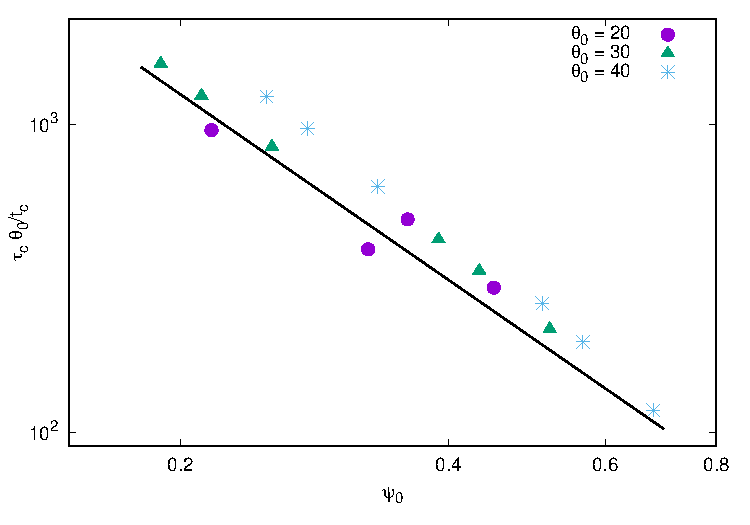
\includegraphics[width=0.85\linewidth]{tauc_vs_psi0_alpha2.pdf}
    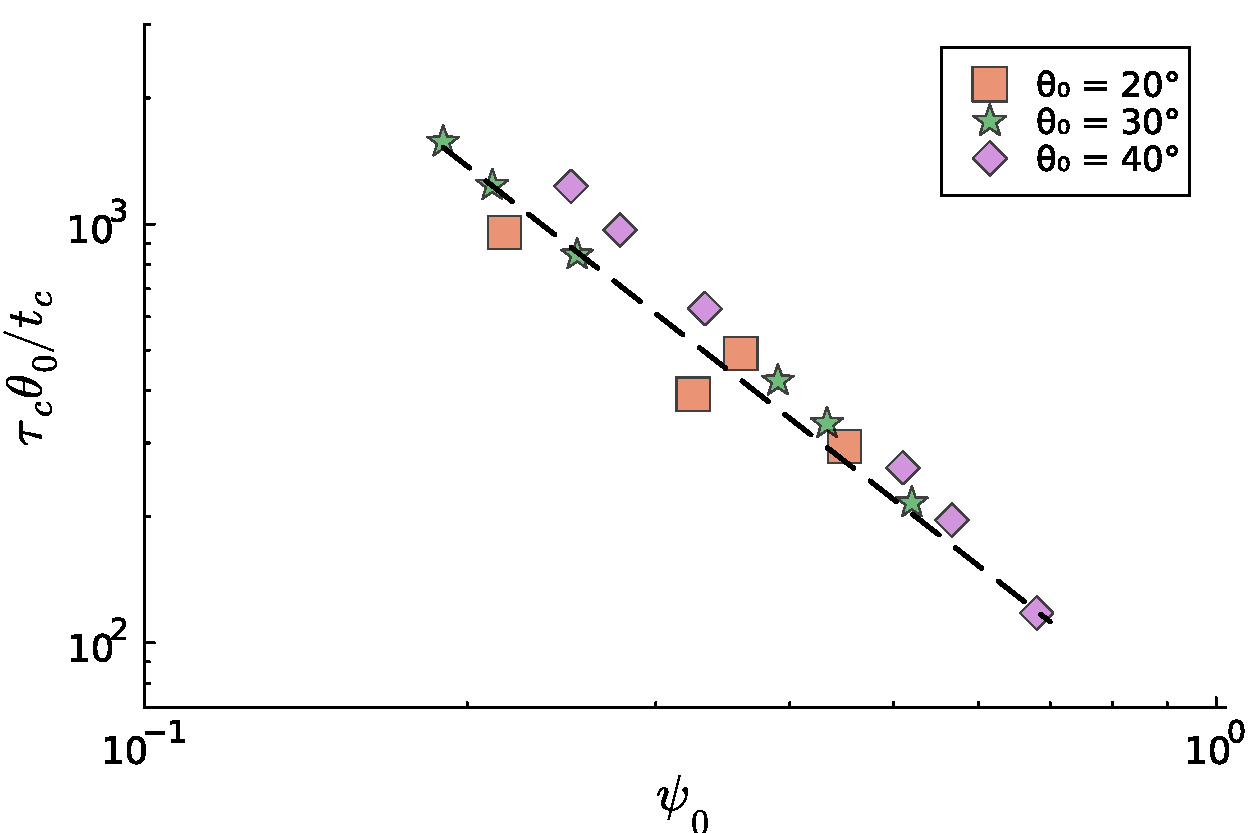
\includegraphics[width=0.85\linewidth]{psi_0_collapse_thetapow1.pdf}
    \caption{Collapse time vs initial aspect ratio for different substrate 
    contact angles. The solid line is the prediction (\ref{eq:tauctheo}) 
    for $\alpha=2$.}
    \label{fig:tauc_vs_psi0}
\end{figure}
In the revised version we have rephrased the text and made the new figure 4 according to this discussion.
}


\item[ \textbf{\underline{Comment 7.}}]
{
Although the introduction of the paper is reasonable, the authors do not mention previous work on radial and angular variation of wettability for drops~\cite{Savva_Groves_Kalliadasis_2019} that may be relevant for section 3.2.
}

\item[ \textbf{{Answer}}] 
{
We thank the Referee for suggesting this relevant reference. We have included it  both in the introduction, among the cited literature where we mention that "a number of studies have focused on thin film dewetting and droplet transport on patterned substrates", and in section IIIB where we have added the following 
comment, when we introduced the linear wettability gradient:\\
\\
\textcolor{red}{the idea of using linear wettability gradients was proposed originally to steer droplet motion \cite{Savva_Groves_Kalliadasis_2019}}.

}

\item[ \textbf{\underline{Comment 8.}}]
{
Fig. 5 is a mess and difficult to understand, probably because the parameter $r_m$ is absent. However, the comments about the approximate formula (6) being at odds with the results have the same drawbacks as those in the previous section.
}

\item[ \textbf{{Answer}}]
{
We provide now values of $r_m$ (see answer to comment 3). But, as discussed 
there, in all cases we are well within the large initial mean radius limit. 
Therefore, as in the uniform case, we do not believe that the mismatch with the LSA
(if any) should be attributed to the values of the $r_m$.
We would like to remark, also, for the sake of clarity, that the "at odds" in 
section IIIB.1 is not in comparison to the LSA, but to the uniform case.
We say, in fact, {\it "at odds with the uniform case (see Fig. 2), moreover, the data correlates less with the LSA prediction $n_d = \pi/(2\psi_0)$"}, implying that it does correlate well in the uniform case (at least up to $\psi_0 \approx 0.2$).
}

\item[ \textbf{\underline{Comment 9.}}]
{
The results about the annular band are interesting as a way to deter the collapse. 
I wonder if this explains why the breakup is faster than in the uniform case, since the energy invested in the collapse is now transferred to the breakup. 
Could the authors show the evolution of the amplitudes of the collapse (axisymmetric) and the breakup (non axisymmetric perturbations) as time evolves? 
This could help in understanding the reasons of the observed behaviour. 
}

\item[ \textbf{{Answer}}]
{
This is indeed a very interesting remark. Actually, the observed phenomenology is even more complicated. In fact, the breakup times are shorter on the annular band only for the lowest band contact angle $\theta_a$, i.e. for the largest
wettability contrast (when, then, the confinement is more effective, thus 
going in the direction suggested by the Referee), and for very low aspect-ratios ($\psi_0 \leq 0.05$). For larger $\theta_a$ and $\psi_0$, the $\tau_b$'s are larger on the annular band than on the uniform substrate. It is not easy to disentangle 
the various effects coming at play, although a mode-analysis as the one suggested
by the Referee might help. But it goes, somehow, beyond the scope of this first explorative study. 
We have left, then, this issue as open, adding the following comment at the end 
of section IIIB.1:\\
\\
\textcolor{red}{For large $\theta_a$, i.e. small contact angle contrast, hence when the constraint on the band is less effective, the breakup time grows with $\psi_0$. 
As $\theta_a$ decreases, the overall picture becomes more complicated.
A stronger confining effect decouples radial dynamics and dewetting and $\tau_b$ tends to become almost independent of $\psi_0$, but determined, instead, by the local contact angle. 
In most cases, the breakup times are larger than in the uniform substrate case (cf. 3), suggesting that the annular band pattern makes the ring rivulet slightly more stable against rupture. However, for the lowest
$\theta_a$ and for very low initial aspect-ratios ($\psi_0 \leq 0.05$), the opposite is true, i.e. breakup times are shorter than their counterpart on uniform substrate. This might be probably ascribed to the fact that an effective removal of the collapse mode sets the breakup onto modes with larger wavenumber that, for small $\psi_0$, display shorter breakup times \cite{gonzalezStabilityLiquidRing2013}. This said, a more quantitative and satisfactory explanation of the observed phenomenology requires certainly a deeper investigation, that goes, however, beyond the scope of the present study.}

}

\item[ \textbf{\underline{Comment 10.}}]
{
With respect to the wettability radial profile, the authors observe a faster collapse competing with the breakup for $\theta_b>\theta_a$ . The collapse is probably best modeled by a quasi-static model of the type developed in \cite{gonzalezStabilityLiquidRing2013}, since as the time evolves the conditions for equilibrium are changed by the variations of the contact angles. This, in turn, changes the aspect ratios and $r_m$ leading to faster or slower local growth rates of the mode $n=0$. I think the authors should discuss in more detail why the gradients affect the retraction, since this is an interesting method to control the formation and location of the drops. 
}

\item[ \textbf{{Answer}}]
{
We thank the Referee for this suggestion concerning the theoretical 
interpretation of our observations. In this spirit, we have included two, we think, explanatory sentences in the paragraph related to the positive contact angle gradient; first we write, explicitly, that the pattern is such that\\
\\
\textcolor{red}{the wettability gradient acts as a sort of effective attraction force, favouring ring retraction};\\
\\
secondly we comment on the control on the number of formed droplet
as follows:\\
\\
\textcolor{red}{This phenomenology can be better understood under the light of a quasi-static analysis of the equations of motion \cite{gonzalezStabilityLiquidRing2013}, whereby the breakup mode is selected 
by the instantaneous aspect-ratio $\psi(t)$ and mean radius $R_0(t)$, thus 
explaining the lower number of droplets formed with respect to the uniform 
substrate case for the same $\psi_0$ (where we had, approximately $n_d \approx O(20)$).}
}
\end{itemize}


\bibliographystyle{abbrv}
\bibliography{referees}

\end{document}